\chapter*{Avant-propos -- Les méthodes agiles: une réponse à un malaise ?}\label{avantPropos}
	\addcontentsline{toc}{chapter}{Avant-propos -- Les méthodes agiles: une réponse à un malaise ?}
	\nouveauChapitre
	Un étude à montré que les projets informatiques ont tendance à ne pas aboutir ou à couter beaucoup plus cher que prévu: 
	\begin{itemize}
		\item 25\% des projets seulement respectent les délais et les budgets
		\item 45\% dépassent le budger ou sont en retard
		\item 28\% sont abandonnés ou voient leur périmètre largement restreint
		\item Combien correspondent à des besoins utilisateurs rééls ?!
	\end{itemize}
	\vspace{3cm}
		\begin{figure}[H]
			\center
		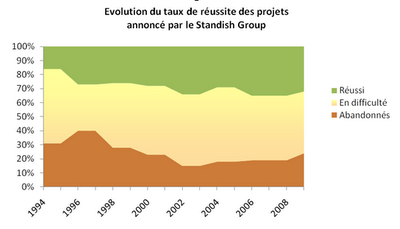
\includegraphics[width=10cm]{images/7-tauxReussite.png}
			\caption{Taux de réussite des méthodes classiques}
		\end{figure}
		\newpage
	\section*{Les causes de ces echecs}
	\addcontentsline{toc}{section}{Les causes de ces echecs}
	Afin de comrendre comment les méthodes Agiles essayent de répondre à ces problèmes, il faut d'abord se demander, pourquoi ces problèmes existent.
	\paragraph{La conformité aux besoins} Les projets ne respectent souvent pas les besoins du client, ou ne comprennent pas ces besoins. Ainsi c'est après des centaines d'heures de développement que le client
	affirme que ce n'est pas ce qu'il voulait.
	\paragraph{Les technologies}
	La technologie choisie pour le projet est extrememnt importante, celle ci doit être capable de permettre de respecter les besoins du client, l'équipe doit la maîtriser, elle doit permettre d'effectuer un développement 
	le plus rapide possible pour ce projet.
	\paragraph{Les méthodes} Les méthodes de développement vont elle aussi également grandement influencé l'avancée du projet, certaines méthodes peuvent permettre de résoudre les problèmes aux plus tôt, mais elle doit
	être adaptée à la taille du projet.
	\newpage
	\section*{Les facteurs clé de l'échec}
	\addcontentsline{toc}{section}{Les facteurs clé de l'échec}
	Les méthodes de développement classiques ont des ponits commun quant à leur raison d'échec. 
	\begin{itemize}
		\item Le manque de communication à tout niveau
		\item Une mauvaise compréhension des besoins
		\item L'insuffisance de l'architecture
		\item L'absence de maturé des outils utilisés
		\item La mauvaise formation des personnes
		\item Le cadre contractuel inadapté
		\item L'insuffisance des tests
	\end{itemize}
	\section*{Les facteurs aidant à la réussite}
	\addcontentsline{toc}{section}{Les facteurs aidant à la réussite}
	Le Standish Group à identifié une dizaine de conditions de succès favorisant la livraison de projets informatiques fructueux.
	Par ordre d'importances, ces conditions sont:
	\begin{enumerate}
		\item L'engagement de la direction
		\item L'implication des utilisateurs
		\item L'expérience du chef de projets
		\item La formulation des objectifs d'affaires
		\item Une envergure limitée aux besoins essentiels
		\item Une infrastructure technologique et stables
		\item Des métholodogies formelles et utilisées
		\item Des estimations fiables et rigoureuses
		\item Autre : découpage des livraisons, compétence du personnel, etc\ldots
	\end{enumerate}
	\section*{Quelques explications de l'échec}
	\addcontentsline{toc}{section}{Quelques explications de l'échec}
	\paragraph{Le client ne maîtrise pas le projet} Le premier problème vient du fait que le client ne maîtrise rien. Il ne connait pas le langage de modélisation utilisé, et se retrouve en conséquence 
	exclue du processus dès la fin des interviews. Également, l'équipe ne va pas lui montrer régulièrement une avancée du projet, or, c'est lui qui sait ce qu'il veut, il pourrait alors mieux préciser ces besoins
	et les problèmes que peuvent comporter le projet au fur et à mesure.
	\paragraph{Cycles de développement trop long} Avoir des cycles de développement court permet de mieux maîtriser l'avancée du projet, tester 
	régulièrement\footnote{Éventuellement avec du développement dirigé par les tests} permet d'éviter de gros prolbèmes de conception. 

	
	


	
		
